%%%%%%%%%%%%%%%%%%%%%%%%%%%%%%%%%%%%% 
%% LE2I beamer template
%% Guillaume Lemaitre, October 2014
%%%%%%%%%%%%%%%%%%%%%%%%%%%%%%%%%%%%% 

\documentclass{beamer}

\usepackage[utf8]{inputenc}
\usepackage[T1]{fontenc} 
\usetheme{le2i} 

%% The amssymb package provides various useful mathematical symbols
\usepackage{amssymb}
%% The amsthm package provides extended theorem environments
\usepackage{amsthm}

%% amsmath for math environment
\usepackage{amsmath}

\DeclareMathOperator*{\argmin}{arg\,min}
\DeclareMathOperator*{\argmax}{arg\,max}
\DeclareMathOperator*{\sign}{sign}

%% figure package
\usepackage{epsf,graphicx}
\usepackage{epstopdf}
\usepackage{subfigure}
\usepackage{transparent}

%% In order to draw some graphs
\usepackage{tikz,xifthen}
\usepackage{tikz-qtree}
\usepackage{adjustbox}
\usetikzlibrary{decorations.pathmorphing}
\usetikzlibrary{fit}
\usetikzlibrary{backgrounds}
\usetikzlibrary{shapes,arrows,shadows}
\usetikzlibrary{calc,decorations.pathreplacing,decorations.markings,positioning}
\usetikzlibrary{snakes,decorations.text,shapes,patterns}
% \usepackage{scalefnt,lmodern,booktabs}

%% Package for cross and tick symbols
\usepackage{pifont}
\newcommand{\tick}{\color{green!60!black!80}\ding{51}}
\newcommand{\cross}{\color{red!60!black!80}\ding{55}}

\title{Image Enhancement\\
Frequency Domain}
\author{Guillaume Lemaitre}
%\date{Define the event \\ day\textsuperscript{th} Month Year}

\institute{Universit\'e de Bourgogne} 

%% Uncomment if you want to avoid thousand of bullet inside the menu
% \usepackage{etoolbox}
% \makeatletter
% \patchcmd{\slideentry}{\advance\beamer@xpos by1\relax}{}{}{}
% \def\beamer@subsectionentry#1#2#3#4#5{\advance\beamer@xpos by1\relax}%
% \makeatother

\begin{document}

% Show the title page
\begin{frame}
  \titlepage
\end{frame}

% Show the table of contents
\begin{frame}
  \tableofcontents[sectionstyle=show,subsectionstyle=show,subsubsectionstyle=hide]
\end{frame}

%---------------------
\section{Fundamentals}
\begin{frame}
\frametitle{Fundamentals}
\begin{block}{Fourier Series}
\begin{itemize}
	\item A \textbf{periodic} function which is represented by the sum of $\sin$ and $\cos$ of different frequencies and multiplied by a different coefficient	
\end{itemize}
\end{block}
\begin{block}{Fourier Transform}
\begin{itemize}
	\item A \textbf{non-periodic} function which is represented by the integral of $\sin$ and $\cos$, by weighing function
\end{itemize}
\end{block}
\end{frame}
%-----------------
\section{Introduction}
\begin{frame}
\frametitle{Introduction to Fourier Transform}
\begin{block}{Fourier transform of continuous function $f(x)$}
\begin{itemize}
	\item $f(x)$, continuous function of real variable $x$
	\item []
	$$\Im\lbrace f(x)\rbrace = F(u) = \int\limits_{-\infty}^{\infty} f(x) exp[-2j\pi ux] dx$$
	\noindent where $j = \sqrt{-1}$ and $u$ is the frequency variable
	\item Integral shows $F(u)$ composed of infinite sum of sine and cosine 
	\item Each $u$ value determines the frequency of its corresponding $\sin$ and $\cos$ pair
\end{itemize}
\end{block}
\end{frame}
%----------
\begin{frame}
\frametitle{Introduction to Fourier Transform}
\begin{block}{Inverse Fourier transform of $F(u)$}
\begin{itemize}
	\item Having $F(u)$, $f(x)$ can be obtained by the inverse Fourier transform
	\item []
	$$\Im^{-1}\lbrace f(u)\rbrace = f(x) = \int\limits_{-\infty}^{\infty} F(u) exp[2j\pi ux] du$$
\end{itemize}
\end{block}

\begin{itemize}
\item The above equations represent the Fourier transform pair
\end{itemize}
\end{frame}
%----------
\begin{frame}
\frametitle{Introduction to Fourier Transform}
\begin{block}{Fourier transform pair for $f(x,y)$ of two variables}
	$$\Im\lbrace f(x,y)\rbrace = F(u,v) =\int \int\limits_{-\infty}^{\infty} f(x,y) exp[-2j\pi (ux+vy)] dx dy$$
	$$\Im^{-1}\lbrace F(u,v)\rbrace = f(x,y) =\int \int\limits_{-\infty}^{\infty} F(u,v) exp[-2j\pi (ux+vy)] du dv$$
	\noindent $u$ and $v$ are the frequency domain
\end{block}
\end{frame}
%----------
\begin{frame}	
\frametitle{Introduction to Fourier Transform}
\framesubtitle{Discrete Fourier Transform (DFT), discrete signal}
\begin{block}{Fourier transform pair - 1D}
\small{
	$$F(u) = \frac{1}{M}\sum^{M-1}_{x=0} f(x) exp[-2\pi ux/M]$$ \vspace{0.1cm} for $u = 0, 1, 2, ..., M-1$
	}
\small{
	$$f(x) = \sum^{M-1}_{u=0} f(u) exp[2\pi ux/M]$$ \vspace{0.1cm} for $x = 0, 1, 2, ..., M-1$
	}		
\end{block}
\end{frame}
%----------
\begin{frame}	
\frametitle{Introduction to Fourier Transform}
\framesubtitle{Discrete Fourier Transform (DFT)}
\begin{block}{Fourier transform pair - 2D}
\small{
	$$F(u,v) = \frac{1}{MN} \sum^{M-1}_{x=0}\sum^{N-1}_{y=0} f(x,y) exp[-2\pi (ux/M + uy/N)]$$ \vspace{0.1cm} for $u = 0, 1, 2, ..., M-1$, and $v = 0, 1, 2, ..., N-1$ 
	}
\small{
	$$f(x,y) = \sum^{M-1}_{u=0} \sum^{N-1}_{v=0} f(u,v) exp[2\pi (ux/M+uv/N)]$$ \vspace{0.1cm} for $x = 0, 1, 2, ..., M-1$ and $y = 0, 1, 2, ..., N-1$
	}		
\end{block}
\end{frame}
%----------
\begin{frame}
\frametitle{Introduction to Fourier Transform}
\framesubtitle{Discrete Fourier Transform (DFT)}
\begin{itemize}
	\item The Fourier transform of a real function is generally complex and we use polar coordinates: 
\end{itemize}
\begin{columns}
\column{0.5\textwidth}
\begin{block}{1D - DFT}
\scriptsize{
$$F(u) = R(u)+jI(u)$$
$$F(u) = \vert F(u) \vert e^{j \phi (u)} $$
Magnitude spectrum:
$$\vert F(u) \vert = [R^{2}(u)+ I^{2}(u)]^{0.5}$$
Phase spectrum:
$$ \phi (u) = \tan^{-1} \left[ \frac{I(u)}{R(u)} \right] $$
}
\end{block}
\column{0.5\textwidth}
\begin{block}{2D - DFT}
\scriptsize{
$$F(u,v) = R(u,v)+jI(u,v)$$
$$F(u,v) = \vert F(u,v) \vert e^{j \phi (u,v} $$
Magnitude spectrum:
$$\vert F(u) \vert = [R^{2}(u,v)+ I^{2}(u,v)]^{0.5}$$
Phase spectrum:
$$ \phi (u,v) = \tan^{-1} \left[ \frac{I(u,v)}{R(u,v)} \right] $$
}
\end{block}
\end{columns}			
\end{frame}
%----------
\begin{frame}
\frametitle{Introduction to Fourier Transform}
\framesubtitle{Discrete Fourier Transform (DFT)}
\begin{block}{2D- DFT - Basic properties}
\begin{itemize}
\scriptsize{
	\item Power spectrum: 
	$$P(u,v) = \vert F(u,v)^2 \vert $$
	\item Average gray level of the image: 
	$$F(0,0) = \frac{1}{MN}\sum^{M-1}_{x=0}\sum^{N-1}_{y=0} f(x,y)$$
	\item Symmetric spectrum: 
	$$F(u,v) = F*(-u,-v) $$
	$$\vert F(u,v) \vert  = \vert F(-u,-v) \vert $$
}
\end{itemize}
\end{block}
\end{frame}
%----------
\begin{frame}
\frametitle{Introduction to Fourier Transform}
\framesubtitle{Discrete Fourier Transform (DFT)}
\begin{block}{Phase and Magnitude Spectrum}
\centering{

\includegraphics[width= 0.25\textwidth, height = 0.25\textheight]{images/F1_ex2_original.png} \hfill
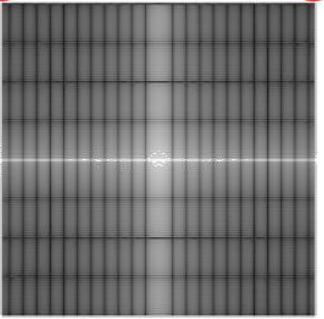
\includegraphics[width= 0.25\textwidth, height = 0.25\textheight]{images/F1_ex2_Mag.png} \hfill
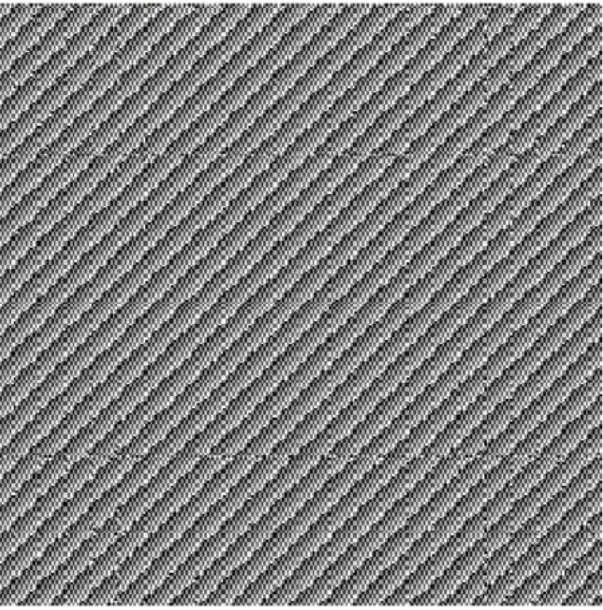
\includegraphics[width= 0.25\textwidth, height = 0.25\textheight]{images/F1_ex2_Phase.png}\\
}
\hspace{-0.7cm} Original \hspace{1.8cm} magnitude \hspace{2.5cm} phase
\end{block}
\end{frame}
%----------
\begin{frame}
\frametitle{Introduction to Fourier Transform}
\framesubtitle{Discrete Fourier Transform (DFT)}
\begin{itemize}
\scriptsize{
	\item Magnitude spectrum tells the amplitude of the sinusoids that forms the image
	\item For any given frequency, large amplitude indicates high influence of that frequency, while the low amplitude indicate the opposite 
	\item Phase indicate the displacement of the sinusoids with respect to their origin 
	\item Effect of magnitude, phase = 0 }
	\begin{center}
	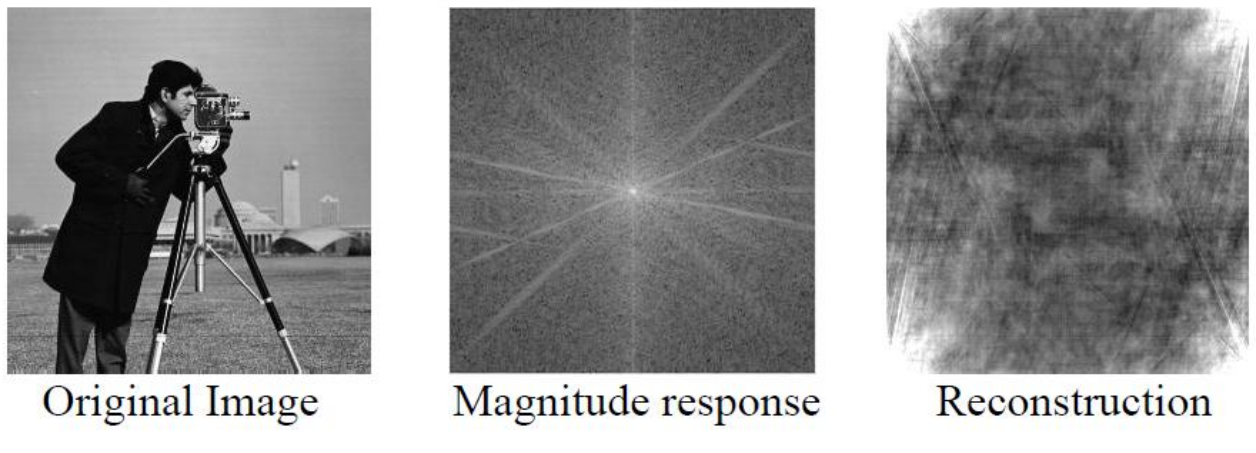
\includegraphics[scale=0.15]{images/F1_MagnitudePhase1.png}
	\end{center}
	\item \scriptsize{Effect of phase, magnitude = constant (80)}
	\begin{center}
	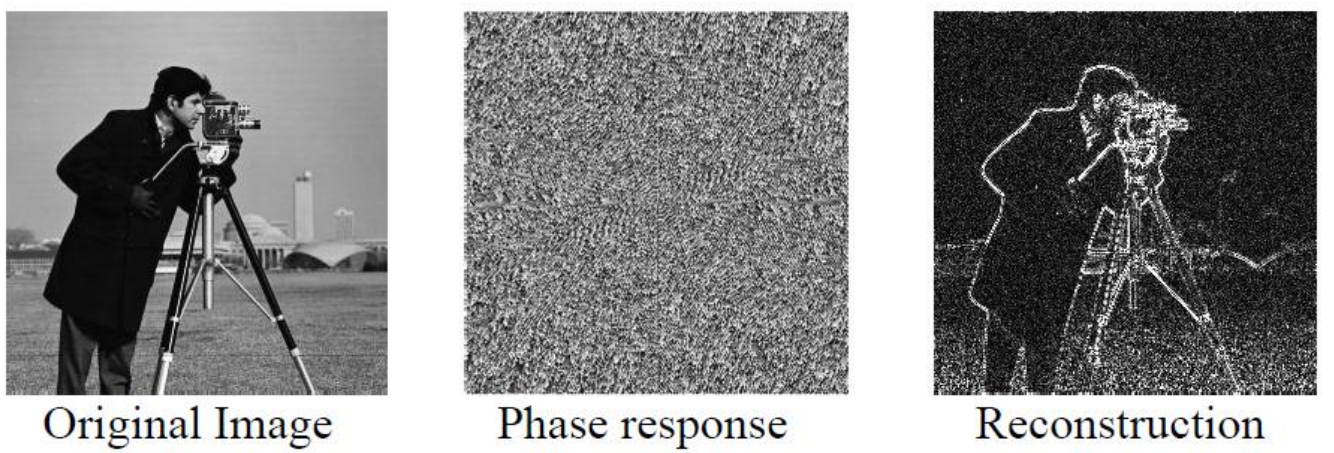
\includegraphics[scale=0.15]{images/F1_MagnitudePhase2.png}
	\end{center}	
\end{itemize}
\end{frame}
%----------
\subsection{DFT Properties}
\begin{frame}
\frametitle{Introduction to Fourier Transform}
\framesubtitle{DFT properties}
\begin{block}{Effect of Translation in Spatial Domain}
\begin{itemize}
\item [] $$ f(x-x{0}, y-y_{0}) \Leftrightarrow F(u,v)e^{-j2\pi(\frac{x_{0}u}{M} + \frac{y_{0}v}{N})}$$
\centering{
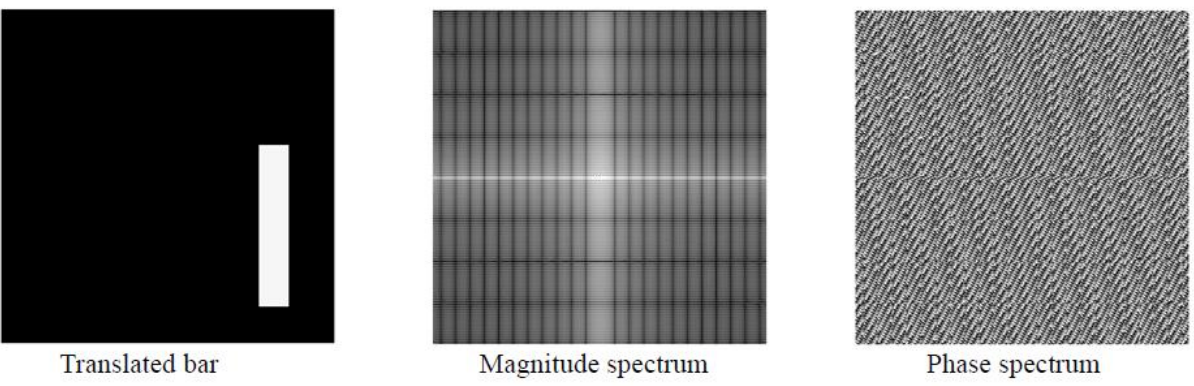
\includegraphics[scale = 0.2]{images/F1_ex2_OriMagPhase_translation.png}
\item A shift in spatial domain, does not affect the magnitude in frequency domain  
}
\end{itemize}
\end{block}
\end{frame}
%----------
\begin{frame}
\frametitle{Introduction to Fourier Transform}
\framesubtitle{DFT Properties}
\begin{block}{Effect of rotation in Spatial Domain}
\begin{itemize}
\scriptsize{
\item [] Considering the polar form i.e. 
$$f(x,y)\Leftrightarrow f(r, \theta)$$ 
$$F(u,v)\Leftrightarrow F( w, \varphi)$$
$$f(r, \theta+\theta_{0}) \Leftrightarrow F(w,\varphi+\theta)$$
\centering{
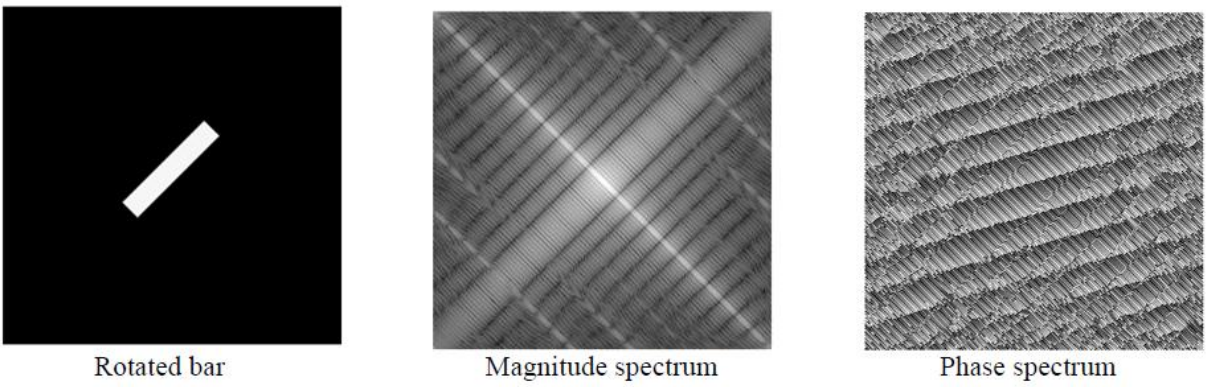
\includegraphics[scale = 0.2]{images/F1_ex2_OriMagPhase_rotation.png} 
}
\item Rotating $f(x,y)$ by $\theta$ rotates $F(u,v)$ by the same angle and vice versa.
}
\end{itemize}
\end{block}
\end{frame}
%---------
\begin{frame}
\frametitle{Introduction to Fourier Transform}
\framesubtitle{DFT Properties}
\begin{block}{Distributing and Scaling}
\scriptsize{
\begin{itemize}
\item Distributive over addition but not over multiplication
$$\Im\lbrace f_{1}(x,y)+f_{2}(x,y)\rbrace = \Im\lbrace f_{1}(x,y) \rbrace +\Im\lbrace f_{2}(x,y)\rbrace $$ 
$$\Im\lbrace f_{1}(x,y).f_{2}(x,y)\rbrace \neq \Im\lbrace f_{1}(x,y) \rbrace .\Im\lbrace f_{2}(x,y)\rbrace $$ 
\item For two scalars a and b 
$$ af(x,y)\Leftrightarrow aF(u,v) $$ 
$$ f(ax,by) \Leftrightarrow \frac{1}{\vert ab \vert} F(u/a, v/b)$$ 
\end{itemize}
}
\end{block}
\end{frame}
%---------
\begin{frame}
\frametitle{Introduction to Fourier Transform}
\framesubtitle{DFT Properties}
\begin{block}{Periodicity and Conjugate Symmetry}
\tiny{
\begin{itemize}
\item The DFT and its inverse are periodic with period $N$
\item[] $$F(u,v) = F(u+M,v) = F(u, v+N) = F(u+M, v+N) $$ 
\item Conjugate symmetry
\item[] $$ F(u,v) = F*(-u,-v)$$ 
\item[] $$ \vert F(u,v) \vert = \vert F(-u,-v)\vert $$
\end{itemize}
}
\end{block}
\begin{block}{Separability}
\tiny{
\begin{itemize}
\item DFT pair can be expressed in separable forms: 
$$F(u,v) = \frac{1}{M}\sum^{M-1}_{x=0} F(x,v) exp[-j2\pi ux/M]$$
$$F(x,v) = \left[ \frac{1}{N}\sum^{N-1}_{y =0} f(x,y)exp[-2\pi vy/N]\right]$$
\end{itemize}}
\end{block}
\end{frame}
%---------
\begin{frame}
\frametitle{Introduction to Fourier Transform}
\framesubtitle{DFT Properties}
\begin{block}{Separability}
\scriptsize{
\begin{itemize}
\item For each value of $x$, the expression inside the brackets is a 1-D transform
\item 2-D $F(x,v)$ is obtained by taking a transform along each row of $f(x,y)$ and multiplying the result by N 
\item $F(u,v)$ is obtained by making a transform along each column of $F(x,v)$
\item[]
\centering{
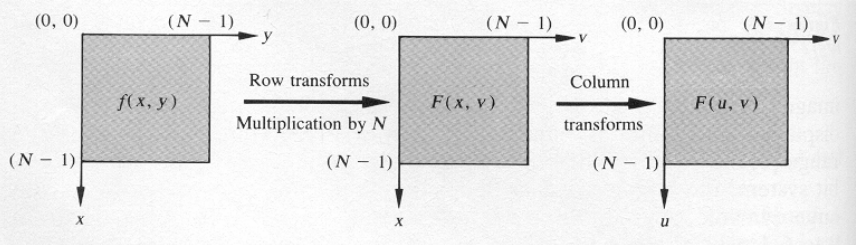
\includegraphics[scale=0.3]{images/F1_Separability}}
\end{itemize}
}
\end{block}
\end{frame}
%---------
\begin{frame}
\frametitle{Introduction to Fourier Transform}
\framesubtitle{DFT Properties}
\begin{block}{Convolution}
\begin{itemize}
\item Convolution theorem with FT pair: 
$$f(x)^\ast g(x) \Leftrightarrow F(u)G(u)$$
$$f(x)g(x) \Leftrightarrow F(u)^\ast G(u)$$
\item Discrete equivalent: 
$$f_{e}(x)^\ast g_{e}(x) = \frac{1}{M} \sum^{M-1}_{m=0}f_{e}(m)g_{e}(x-m)$$ 
\end{itemize}
\end{block}
\end{frame}
%----------
\begin{frame}
\frametitle{Introduction to Fourier Transform}
\framesubtitle{DFT Properties}
\begin{block}{Correlation}
\begin{itemize}
\item Convolution theorem with FT pair: 
$$f(x,y) \circ g(x,y) \Leftrightarrow F^\ast(u,v)G(u,v)$$
$$f^\ast(x,y)g(x,y) \Leftrightarrow F(u,v) \circ G(u,v)$$
\item Discrete equivalent: 
$$f_{e}(x)\circ g_{e}(x) = \frac{1}{M} \sum^{M-1}_{m=0}f_{e}^{\ast}(m)g_{e}(x-m)$$ 
\end{itemize}
\end{block}
\end{frame}
%----------
\section{Image Enhancement}
\begin{frame}
\frametitle{Image Enhancement}
\framesubtitle{Basic Filtering in Frequency Domain}
\begin{itemize}
	\item[]
	\begin{center}
	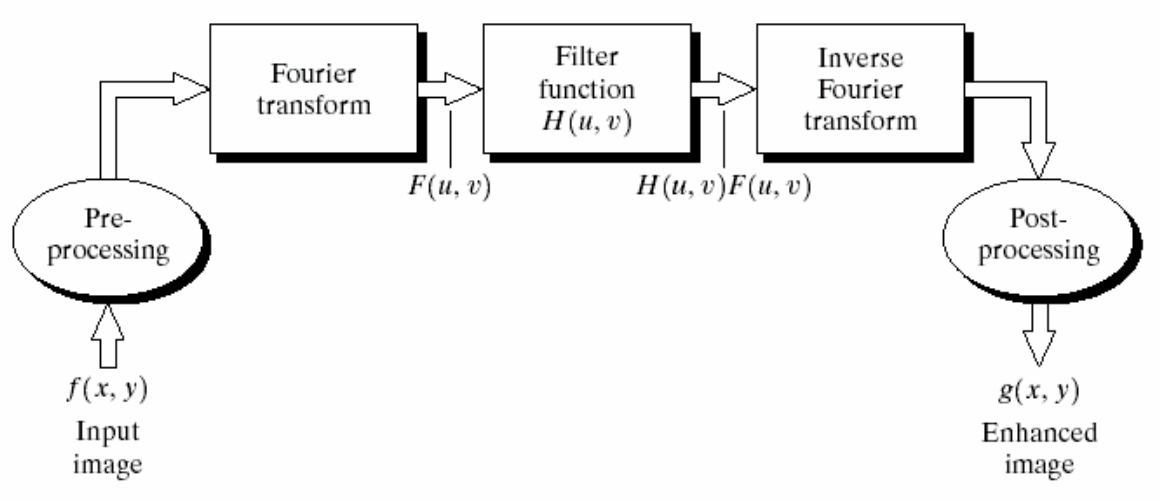
\includegraphics[width = 0.6\textwidth, height = 0.22\textheight]{images/F1_steps.png}
	\end{center}
	\scriptsize{
	\item Compute Fourier transform of image $F(u,v)$
	\item Multiply the result by a filter transfer function $H(u,v)$
	\item Take the inverse transform to produce the enhanced image 
	$$G(u,v) = H(u,v) F(u,v)$$
	$$g(x,y) = \Im^{-1}[G(u,v)] $$
	}
\end{itemize}
\scriptsize{	
\begin{block}{Attention!!}
Because of periodicity when taking DFT we have to avoid wraparound error or aliasing
\end{block}}
\end{frame}
%----------
\begin{frame}
\frametitle{Image Enhancement}
\begin{block}{2D- DFT example}
\begin{center}
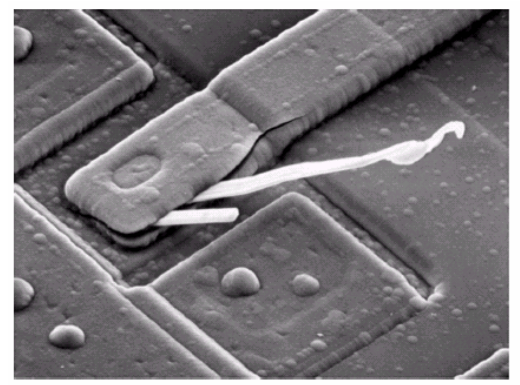
\includegraphics[scale= 0.3]{images/F1_ex_original.png}\
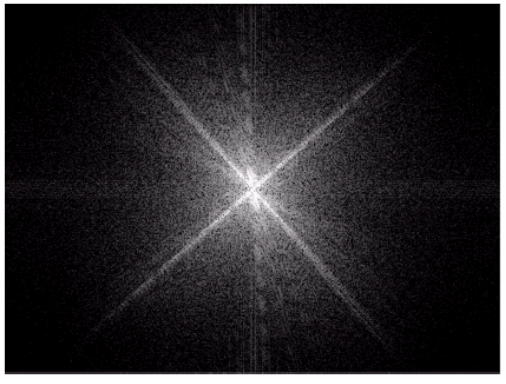
\includegraphics[scale= 0.3]{images/F1_ex_FS.png}
\end{center} 
\scriptsize{SEM image of a damaged integrated circuit}  \quad \quad \scriptsize{Fourier spectrum}
\end{block}
\end{frame}
%----------
\begin{frame}
\frametitle{Image Enhancement}
\framesubtitle{Zero-padding}
{\color{red} You need to add this section}
\end{frame}
%----------
\begin{frame}
\frametitle{Image Enhancement}
\framesubtitle{Filtering}
\begin{block}{Notch Filter}
\begin{itemize}
	\item It forces the average of the image to be 0 
	\item F(0,0) = 0 and then take the inverse 
	\[
 	H(u,v) = 
  	\begin{cases} 
   	0 & \text{if } (u,v) = M/2, N/2 \\
   	1 & \text{otherwise}
  	\end{cases}
	\]
	\item []
	\begin{center}
	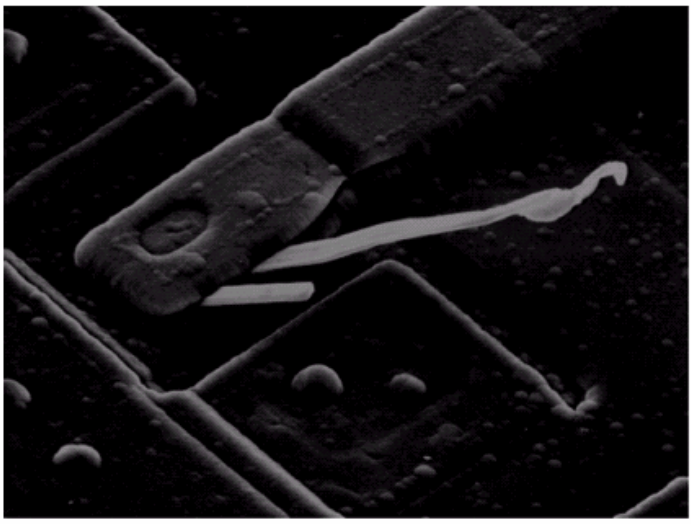
\includegraphics[scale=0.2]{images/F1_ex_notch.png}
	\end{center}
	\item [] \begin{center} Notch filter \end{center}
\end{itemize}
\end{block}
\end{frame}
%---------
\begin{frame}
\frametitle{Image Enhancement}
\framesubtitle{Filtering}
\begin{block}{Low-pass filter}
\begin{itemize}
	\item Reduces the high frequency contents (blurring or smoothing)
	\item []
	\begin{center}
	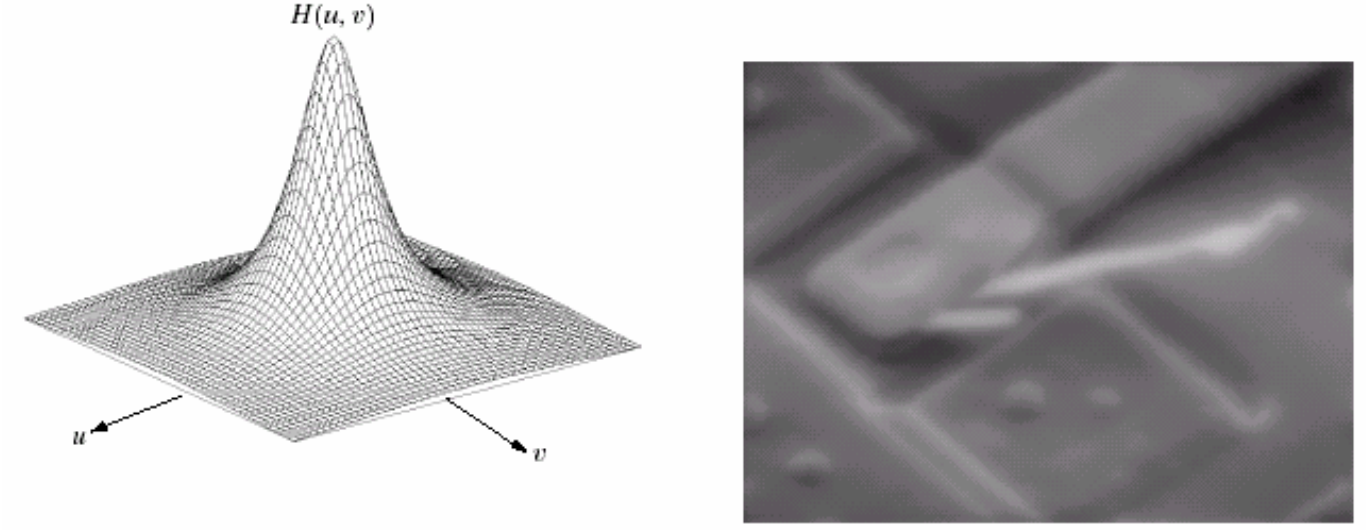
\includegraphics[scale=0.24]{images/F1_ex_LP.png}
	\end{center}
\end{itemize}
\end{block}

\end{frame}
%---------
\begin{frame}
\frametitle{Image Enhancement}
\framesubtitle{Filtering}
\begin{block}{High-pass filter}
\begin{itemize}
	\item Increase the magnitude of the high frequency components relative to low frequency components (sharpening)
	\item []
	\begin{center}
	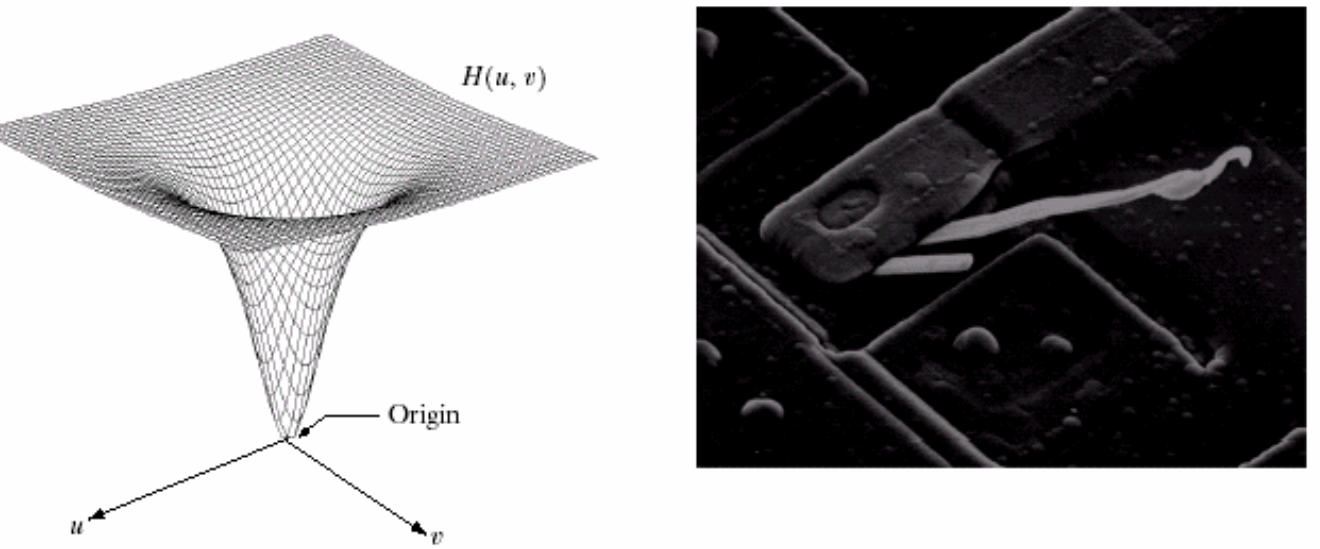
\includegraphics[scale=0.24]{images/F1_ex_HP.png}
	\end{center}
\end{itemize}
\end{block}
\end{frame}
%---------
\subsection{Low-pass filter (Smoothing)}
\begin{frame}
\frametitle{Image Enhancement}
\framesubtitle{Low-pass filter (Smoothing)}
\begin{itemize}
\item Edges, noise contribute significantly to the high-frequency content of the FT of an image
\item Blurring/smoothing is achieved by reducing a specified range of high-frequency components
$$ G(u,v) = H(u,v)F(u,v)$$
\end{itemize}
\begin{block}{Different Types}
\begin{itemize}
\item Ideal 
\item Butterworth
\item Gaussian
\end{itemize}
\end{block}
\end{frame}
%--------
\begin{frame}
\frametitle{Image Enhancement}
\framesubtitle{Low-pass filter}
\begin{block}{Ideal Low-pass filter}
\scriptsize{
\begin{itemize}
\item[] 	\[
 	H(u,v) = 
  	\begin{cases} 
   1 & \text{if } D(u,v) \leq D_{0} \\
   0 & \text{if } D(u,v) > D_{0}
  	\end{cases}
	\]
	\noindent $D_{0}$ is a specified non-negative quantity (Cutoff frequency) \\
	D(u,v) is the distance from point $(u,v)$ to the center of frequency rectangle\\
	$F_{c}(u,v) = (M/2, N/2)$\\
	$D(u,v) = (u^2+v^2)^{1/2}$\\
	\centering{
	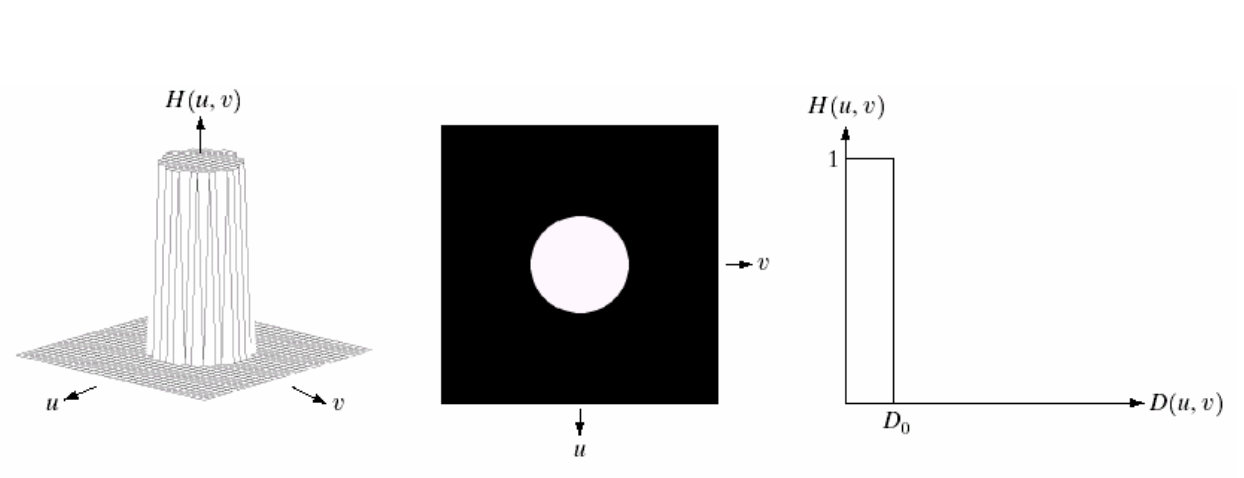
\includegraphics[scale=0.25]{images/F1-LP-Ideal.png}}
\end{itemize}
}
\end{block}
\end{frame}
%---------
\begin{frame}
\frametitle{Image Enhancement}
\framesubtitle{Low-pass filter}
\begin{block}{Ideal low-pass filter}
\scriptsize{Original image and results of ideal low-pass with cutoff frequencies $\{$5,15,30,80,230$\}$}
\centering{
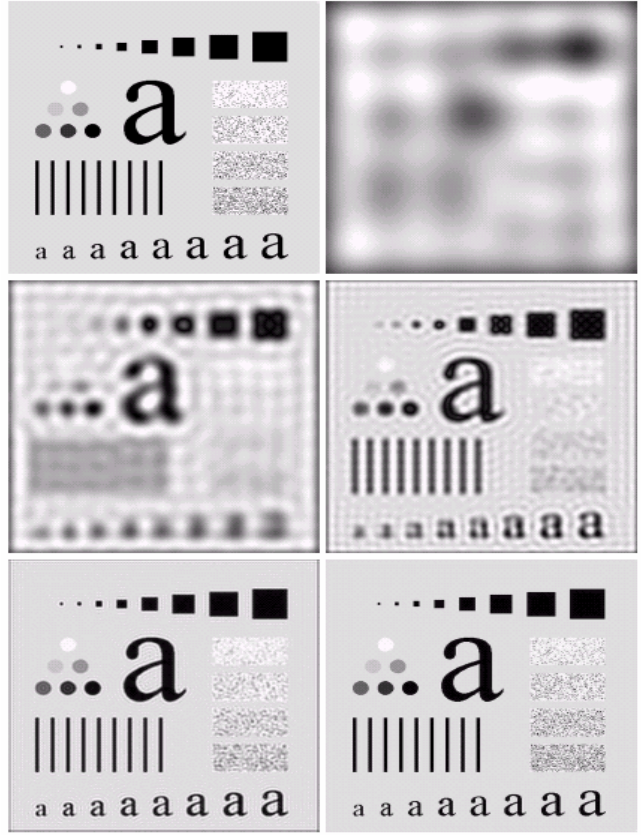
\includegraphics[width= 0.5\textheight, height= 0.6\textheight]{images/F1-ex-LP-ideal.png}
}
\end{block}
\end{frame}
%---------
\begin{frame}
\frametitle{Image Enhancement}
\framesubtitle{Low-pass filter}
\begin{block}{Butterworth low-pass filter}
\scriptsize{
\begin{itemize}
\item[] 	$$ H(u,v) = \frac{1}{1+[D(u,v)/D_{0}]^{2n}}$$

\begin{itemize}
\scriptsize{
	\item $n$ is the order of the filter 
	\item $D_{0}$ cutoff frequency locus (distance from the origin)
	\item $D(u,v) = (u^2 + v^2)^{1/2}$ filter characteristics
	}
\end{itemize}
\item Does not have a sharp discontinuity
\item Does not establish a clear cutoff between passed and filtered frequencies
\item When $D(u,v) = D_{0}$, $H(u,v) = 0.5$\\
	\centering{
	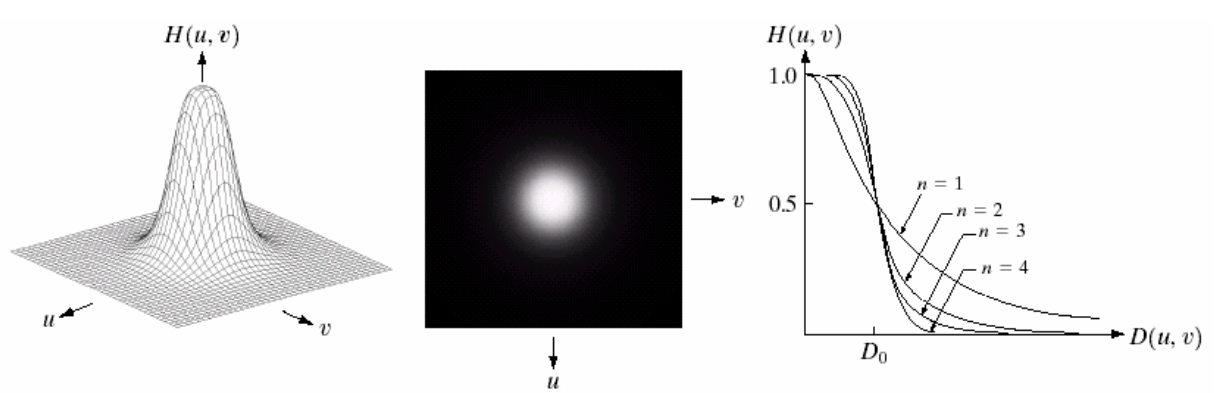
\includegraphics[scale=0.23]{images/F1-LP-BW.png}}	
\end{itemize}
}
\end{block}
\end{frame}
%---------
\begin{frame}
\frametitle{Image Enhancement}
\framesubtitle{Low-pass filter}
\begin{block}{Butterworth low-pass filter}
\scriptsize{Original image and results of Butterworth low-pass with order $2$ and cutoff frequencies $\{$5,15,30,80,230$\}$}\\
\centering{
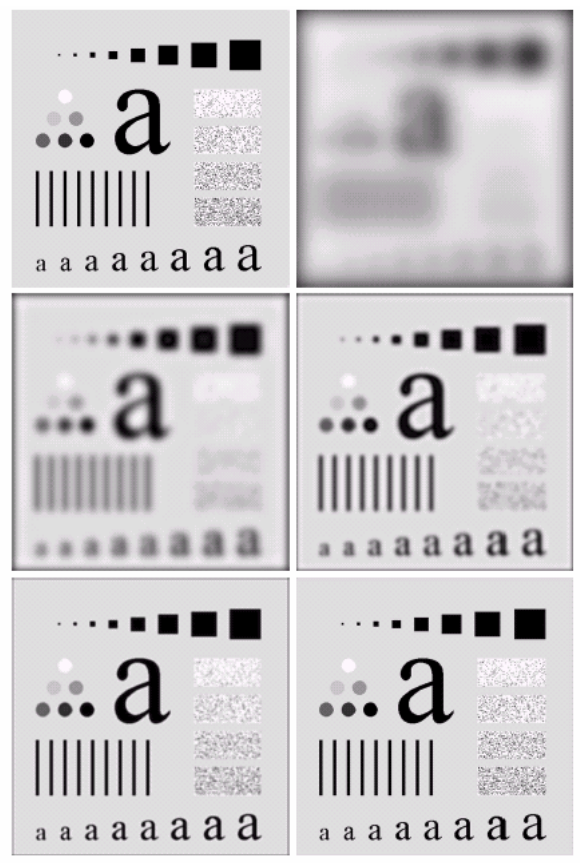
\includegraphics[width= 0.5\textheight, height= 0.6\textheight]{images/F1-ex-LP-BW.png}
}
\end{block}
\end{frame}
%---------
\begin{frame}
\frametitle{Image Enhancement}
\framesubtitle{Low-pass filter}
\begin{block}{Butterworth filter}
\scriptsize{Spatial representation of Butterworth low-pass with orders of $\{$1,2,5,20$\}$}
\centering{
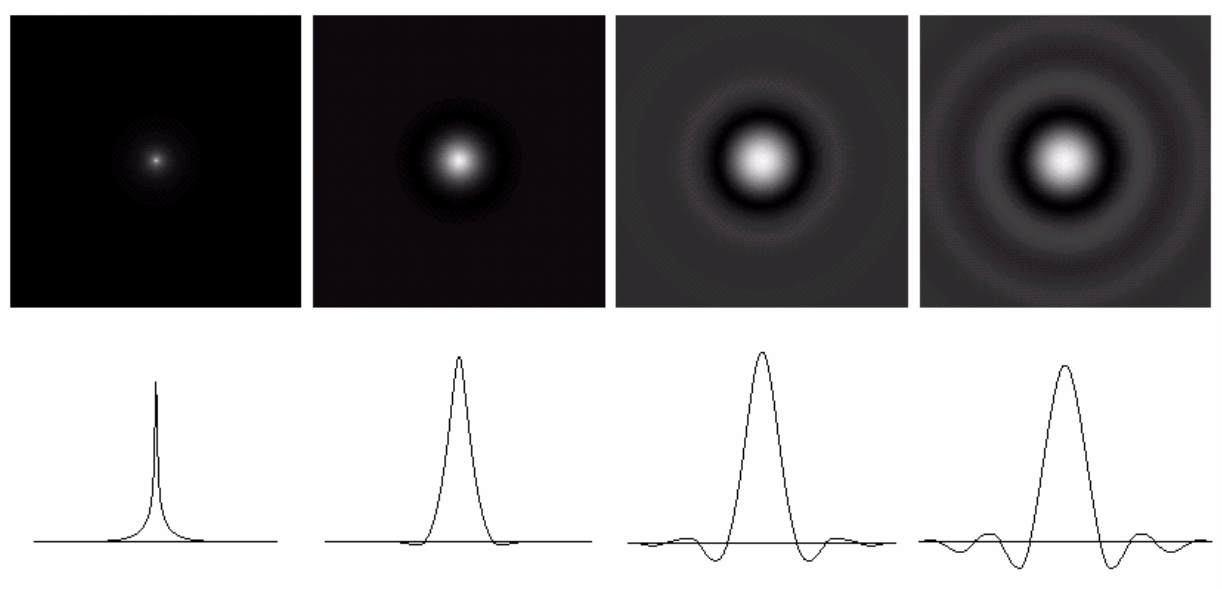
\includegraphics[width= 1.0\textheight, height= 0.5\textheight]{images/F1-ex-LP-BW2.png}
}
\end{block}
\end{frame}
%---------
\begin{frame}
\frametitle{Image Enhancement}
\framesubtitle{Low-pass filter}
\begin{block}{Gaussian low-pass filter}

\begin{itemize}
\item[] 	$$ H(u,v) = e^{-D^{2}(u,v)/2\sigma^{2}}$$ 
\begin{itemize}
	\item $\sigma = D_{0}$ cutoff frequency 
	\item $D(u,v) = (u^2 + v^2)^{1/2}$ Distance from the FT center
\end{itemize}
\item The inverse FT of Gaussian is also a Gaussian\\
	\centering{
	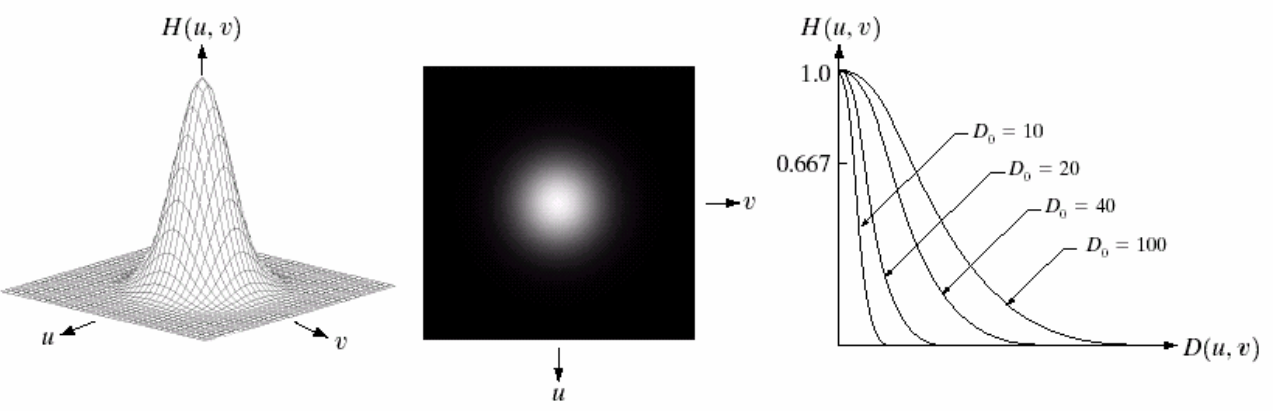
\includegraphics[scale=0.23]{images/F1-LP-Gaussian.png}}	
\end{itemize}

\end{block}
\end{frame}
%----------
\begin{frame}
\frametitle{Image Enhancement}
\framesubtitle{Low-pass filter}
\begin{block}{Gaussian low-pass filter}
\scriptsize{Original image and results of Gaussian low-pass with cutoff frequencies $\{$5,15,30,80,230$\}$}\\
\centering{
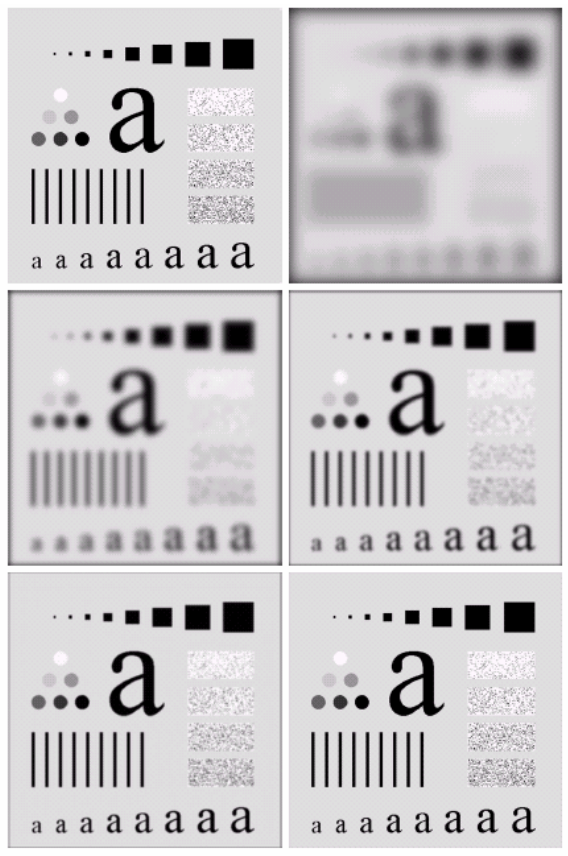
\includegraphics[width= 0.5\textheight, height= 0.6\textheight]{images/F1-ex-LP-Gaussian.png}
}
\end{block}
\end{frame}
%----------
\subsection{High-pass filter (Sharpening)}
\begin{frame}
\frametitle{Image Enhancement}
\framesubtitle{High-pass filter (Sharpening)}
\begin{itemize}
	\item Attenuating low-frequency components without disturbing high-frequency information.
	\item [] $$H_{hp}(u,v) = 1 - H_{lp}(u,v)$$
\end{itemize}
\begin{block}{Different Types}
\begin{itemize}
	\item Ideal 
	\item Butterworth
	\item Gaussian
\end{itemize}
\end{block}
\end{frame}
%-------------
\begin{frame}
\frametitle{Image Enhancement}
\framesubtitle{High-pass filter}
\begin{block}{Ideal High-pass filter}
\scriptsize{
\begin{itemize}
\item[] 	\[
 	H(u,v) = 
  	\begin{cases} 
   0 & \text{if } D(u,v) \leq D_{0} \\
   1 & \text{if } D(u,v) > D_{0}
  	\end{cases}
	\]
\item Opposite of the ideal low-pass\\
	\centering{
	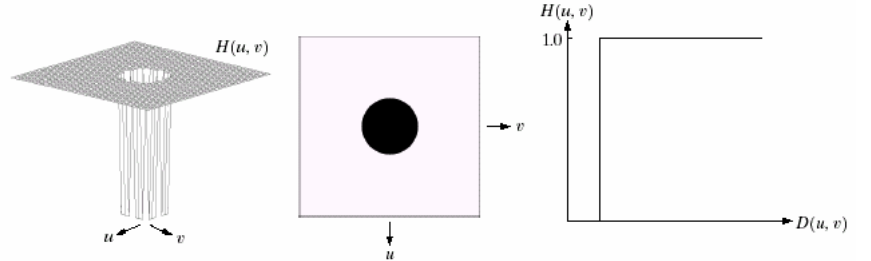
\includegraphics[scale=0.4]{images/F1-HP-Ideal.png}}
\end{itemize}
}
\end{block}
\end{frame}
%-------------
\begin{frame}
\frametitle{Image Enhancement}
\framesubtitle{High-pass filter}
\begin{block}{Butterworth High-pass filter}
\scriptsize{
\begin{itemize}
\item[] 	$$ H(u,v) = \frac{1}{1+[D_{0}/D(u,v)]^{2n}}$$
\item[]
	\centering{
	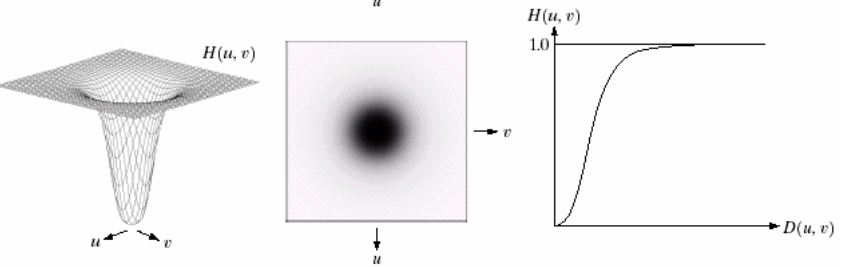
\includegraphics[scale=0.4]{images/F1-HP-BW.png}}	
\end{itemize}
}
\end{block}
\end{frame}
%--------------
\begin{frame}
\frametitle{Image Enhancement}
\framesubtitle{High-pass filter}
\begin{block}{Gaussian High-pass filter}

\begin{itemize}
	\item[] 	$$ H(u,v) = 1 - e^{-D^{2}(u,v)/2\sigma^{2}}$$ 
	\item[]
	\centering{
	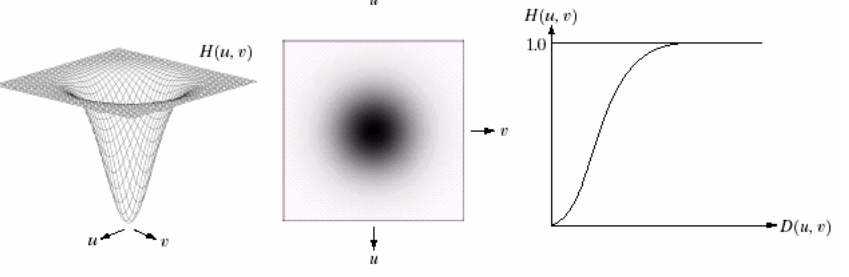
\includegraphics[scale=0.4]{images/F1-HP-Gaussian.png}}	
\end{itemize}
\end{block}
\end{frame}
%----------
\begin{frame}
\frametitle{Image Enhancement}
\framesubtitle{High-pass filter}
\begin{block}{example of Ideal, Butterworth and Gaussian High-pass}

\begin{itemize}
	\item[] \scriptsize{$D_{0} =$ $\{$30, 60, 160 $\}$}
	\item[] \centering{\scriptsize{Ideal High-pass}} \\
	\centering{
	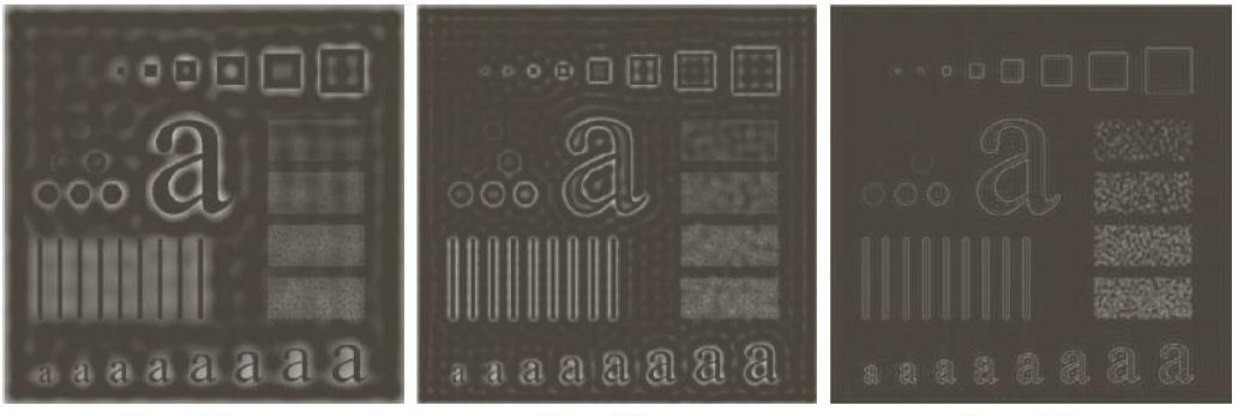
\includegraphics[scale=0.14]{images/F1-ex-HP-ideal.png}}
	\item[] \scriptsize{Butterworth High-pass, $n =2$} \\
	\centering{
	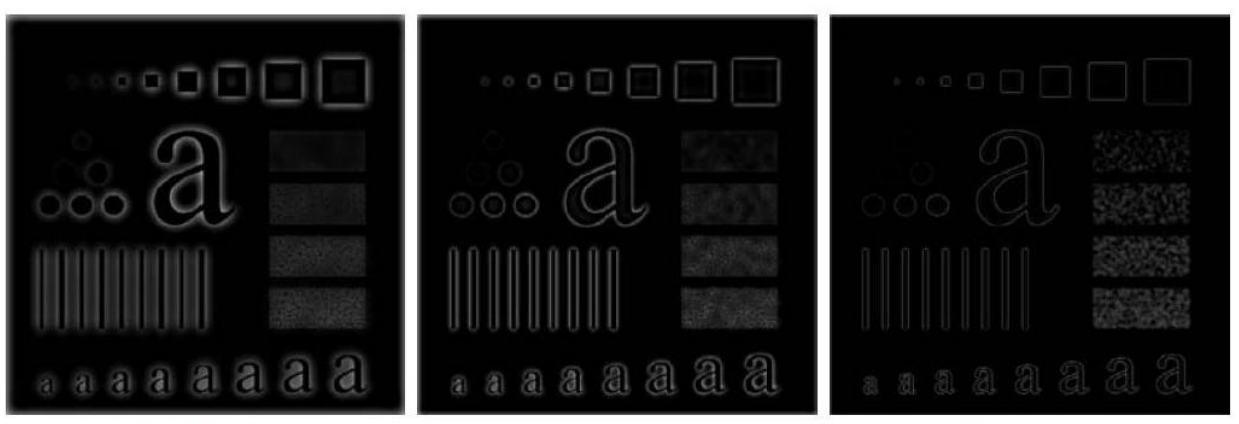
\includegraphics[scale=0.14]{images/F1-ex-HP-BW.png}}	
	\item[] \scriptsize{Gaussian High-pass} \\
	\centering{
	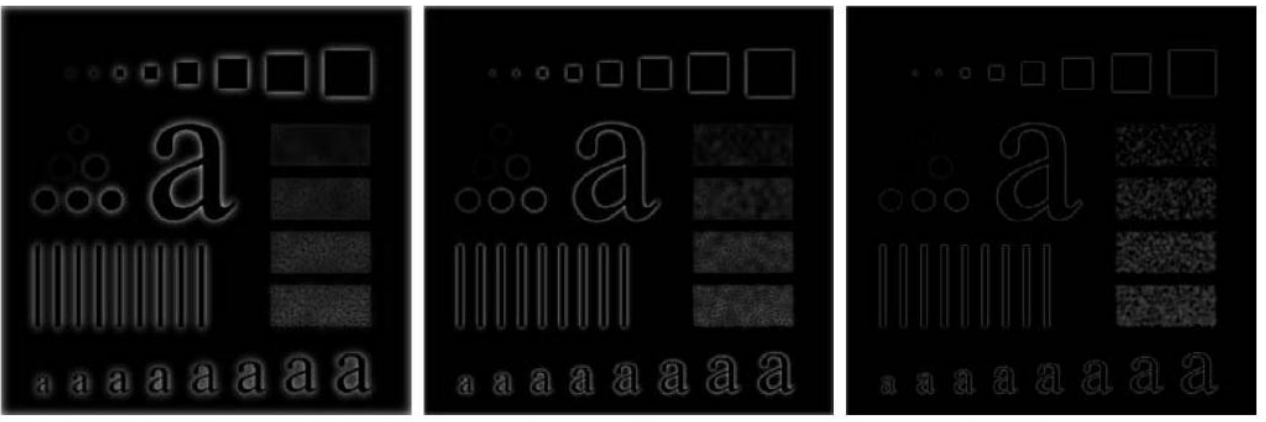
\includegraphics[scale=0.14]{images/F1-ex-HP-Gaussian.png}}		
\end{itemize}
\end{block}
\end{frame}

%-----------
\begin{frame}
\frametitle{Image Enhancement}
\framesubtitle{High-pass filter}
\begin{block}{Recall}
\begin{itemize}
\scriptsize{
	\item[] 	$$ \nabla ^2 f = \frac{\partial^2 f}{\partial x^2} + \frac{\partial^2 f}{\partial y^2}$$ 
	\item[] $$ \nabla ^2 f = \left[f(x+1,y)+f(x-1,y)+f(x,y+1)+f(x,y-1)\right]-4f(x,y)$$ 
	}
\end{itemize}
\end{block}
\begin{block}{Laplacian in FD}
\begin{itemize}
\scriptsize{
	\item[]$$ \Im [\nabla^2 f(x,y)] = -(u^2 +v^2)F(u,v) $$	
	\item[]$\rightarrow$ The Laplacian can be implemented in FD by using a filter 
	\item[] $$ H(u,v) = -(u^2 +v^2) $$ 
	\item FT pair: 
	$$ \nabla^2 f(x,y) \Leftrightarrow [(u-M/2)^2 (v-N/2)^2]F(u,v )$$
	}
\end{itemize}
\end{block}
\end{frame}
%-----------

\end{document}

%\begin{itemize}
%\item Also use neighborhood but do not use coefficients 
%\begin{itemize}
%\item median filter for noise reduction
%\end{itemize} 
%\end{itemize}
